\documentclass[a4paper]{article}

%use the english line for english reports
%usepackage[english]{babel}
\usepackage[portuguese]{babel}
\usepackage[utf8]{inputenc}
\usepackage{indentfirst}
\usepackage{graphicx}
\usepackage{verbatim}
\usepackage[margin=1.0in]{geometry}
\usepackage{listings}
\usepackage{color}

\definecolor{dkgreen}{rgb}{0,0.6,0}
\definecolor{gray}{rgb}{0.5,0.5,0.5}
\definecolor{mauve}{rgb}{0.58,0,0.82}

\begin{document}
\lstset{frame=none,
  language=C,
  aboveskip=3mm,
  belowskip=3mm,
  showstringspaces=false,
  columns=flexible,
  basicstyle={\small\ttfamily},
  numbers=none,
  numberstyle=\tiny\color{gray},
  keywordstyle=\color{blue},
  commentstyle=\color{dkgreen},
  stringstyle=\color{mauve},
  breaklines=true,
  breakatwhitespace=true,
  tabsize=3
}

\renewcommand{\figurename}{Fig.}

\setlength{\textwidth}{16cm}
\setlength{\textheight}{22cm}

\title{\Huge\textbf{First Laboratory Project}\linebreak\linebreak\linebreak
\Large\textbf{Data Link Protocol}\linebreak\linebreak
\linebreak\linebreak

\includegraphics[scale=0.1]{feup-logo.png}\linebreak\linebreak
\linebreak\linebreak
\Large{Master in Computer Engineering and Informatics} \linebreak\linebreak
\Large{Computer Networks}\linebreak
}

\author{\textbf{Grupo:}\\
Carolina Centeio Jorge - up201403090 \\
João Fidalgo - up201303098 \\
Mónica Fernandes - up201404789 \\
Tiago Almeida - up201305665 \\
\linebreak\linebreak \\
 \\ Faculdade de Engenharia da Universidade do Porto \\ Rua Roberto Frias, s\/n, 4200-465 Porto, Portugal \linebreak\linebreak\linebreak
\linebreak\linebreak\vspace{1cm}}

\maketitle
\thispagestyle{empty}

%************************************************************************************************
%************************************************************************************************

\newpage

%Todas as figuras devem ser referidas no texto. %\ref{fig:codigoFigura}
%
%%Exemplo de código para inserção de figuras
%%\begin{figure}[h!]
%%\begin{center}
%%escolher entre uma das seguintes três linhas:
%%\includegraphics[height=20cm,width=15cm]{path relativo da imagem}
%%\includegraphics[scale=0.5]{path relativo da imagem}
%%\includegraphics{path relativo da imagem}
%%\caption{legenda da figura}
%%\label{fig:codigoFigura}
%%\end{center}
%%\end{figure}
%
%
%\textit{Para escrever em itálico}
%\textbf{Para escrever em negrito}
%Para escrever em letra normal
%``Para escrever texto entre aspas''
%
%Para fazer parágrafo, deixar uma linha em branco.
%
%Como fazer bullet points:
%\begin{itemize}
	%\item Item1
	%\item Item2
%\end{itemize}
%
%Como enumerar itens:
%\begin{enumerate}
	%\item Item 1
	%\item Item 2
%\end{enumerate}
%
%\begin{quote}``Isto é uma citação''\end{quote}


%%%%%%%%%%%%%%%%%%%%%%%%%%

\section{Summary}

This laboratory project was done in the scope of the subject Computer Networks of the Master in Computer Engineering and Informatics course in the school year of 2016/2017. All required knowledge and skills were provided both in the theoretical and practical classes of this subject, giving special attention to the Application Layer and Data Link Layer slides. Also, the laboratory guide was an essential tool for the development, as it contained all the requirements and all the necessary guides for this project.

This project's development was extremely important, since it allowed us to understand better how the theoretical concepts are actually applied to real world problems. We concluded that to successfully transfer files between two machines, we must guarantee the integrity of all transfered data and therefore, the usage of a data link protocol is crucial.


\section{Introduction}

In the first few practical classes, we learnt how to transfer supervision frames and how to set up an alarm based on a timeout system, so the transmitter knew when to resend data. The goal of this project was to implement a data link protocol between two computers through a serial port and test it by transferring a gif file, although, due to the fact that the file is read as a binary file, other formats would also be supported. The project was developed in a computer with an operating system based on LINUX, using only the C programming language and RS-232 serial ports with asynchronous communication.

This report will explain in better detail the solution we chose to implement for this problem. In the sections 2 and 3, respectively, we describe the project's architecture and structure of the code. Also, in section 4, we demonstrate the main use cases. In the section 5 and 6, we analyze in detail the data link protocol and application protocol, respectively. In section 7, we describe the tests that were made to validate the program and present some results and finally, in section 8, we declare the appreciation elements that were implemented.

\section{Architecture}

\subsection{Layers}
The main program can be divided in two modules, the \textbf{receiver} and the \textbf{transmitter}. Despite this division, the main program is just one and the user is the one who decides which computer is the transmitter and which one is the receiver by passing it as an argument. 

There are two main layers that allow the program to run correctly called \textbf{application layer} and \textbf{link layer}. The application layer is responsible for the transfer and the reception of files, since it's in this layer that the functions to send and receive data packages are executed. The link layer is responsible for aspects related with the serial port, since it's in this layer that the functions to send and receive supervision and information frames are executed. Although, none of this would be possible with the API functions to write and send frames.

\subsection{Interface}
The user is able to choose the port, the data package size, the number of tries in case of error, the timeout, the file and if the computer is going to behave as the transmitter or the receiver by passing those as arguments when calling the main function. While the program is running, it is displayed in the console every frame that is being sent and received as well as the respective responses. If the transfer is successful, the program will print the size of the received file or, in case of error, it will print an error message with what went wrong. 

\begin{figure}[h!]
	\centering
	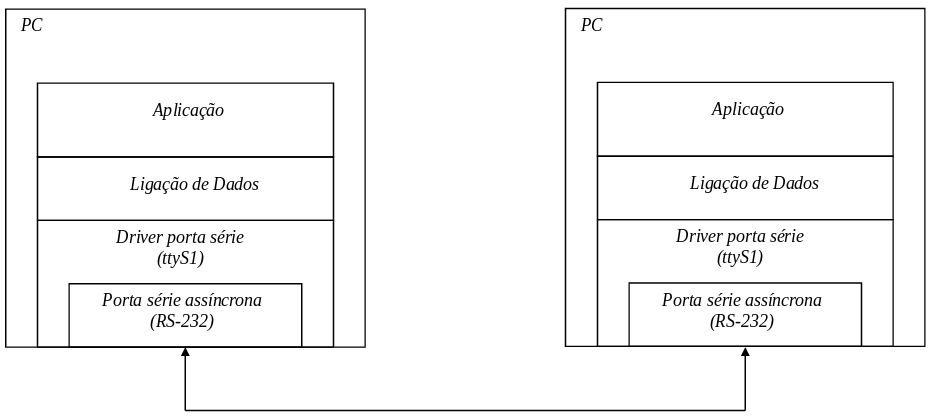
\includegraphics[width=1\textwidth]{Architecture.png}
	\caption{Program Architecture}
	\label{Image: Program Architecture}
\end{figure}

\section{Code Structure}
The application layer is implemented in the files ApplicationLayer.c and ApplicationLayer.h. As suggested in the laboratory guide, we used a struct to store this layer data.

\begin{lstlisting}
struct applicationLayer {
    int fd;
    int status; //Connection mode, 0 - Receiver, 1 - Transmitter
    unsigned int messageSize;
    char* fileName;
};
\end{lstlisting}

The functions of the application layer are:

\begin{lstlisting}
int writeControlPackage(int control, char* fileName, char * fileSize);
int initializeApplicationLayer(char* port, unsigned int messageSize, int retries, int timeout, char* fileName, int status);
int send();
int receive();
\end{lstlisting}

The link layer is implemented in the files LinkLayer.c and LinkLayer.h. Again, as suggest in the laboratory guide, we used a struct to store the data of this layer. 

\begin{lstlisting}
struct linkLayer {
    char port[20];
    unsigned int sequenceNumber;
    unsigned int timeout;
    unsigned int triesMAX;
};
\end{lstlisting}

The functions of the link layer are:

\begin{lstlisting}
void handleAlarm();
int sendMessage(int fd, char* message);
int receiveMessage(int fd, char* message);
int initializeLinkLayer(int fd, char * port, int triesMAX, int timeout);
int llopen(int fd, int connectionMode);
int llwrite(int fd, char* buffer, unsigned int length);
int llread(int fd, char* buffer);
int llclose(int fd, int mode);
unsigned int dataStuffing(char* buffer, unsigned int frameSize);
unsigned int dataDestuffing(char* buffer, unsigned int frameSize);
char findBCC2(char* data, unsigned int size);
\end{lstlisting}

The main function is in the Lab1.c file, where we store the arguments passed by the user and initialize the application layer.

\section{Use Cases}

The program's execution depends on whether the machine is the transmitter or the receiver. However, there are some functions that are executed in both cases, such as \textbf{llopen}, which is used to establish connection between the two machines and \textbf{llclose}, which is used to disconnect the two machines. 

When the program is executed as the transmitter, we open the file for reading using the API function \textbf{open}. After that, we use the function \textbf{writeControlPackge} to send the \textbf{START} package, which uses the \textbf{llwrite} function of the link layer to send the frame. Next, we enter a cycle where the file will continue to be read until there is nothing more to read and in every iteration, a data package is created with the proper header and tail and sent using the \textbf{llwrite} function. Finally, when everything is read, we use the \textbf{writeControlPackage} function to send the \textbf{END} package and close the file with the API function \textbf{close}. 

When the program is executed as the receiver, however, we use the \textbf{llread} function to read the packages sent from the transmitter. Once the \textbf{START} package is read, we open the destination file using the API function \textbf{open} and in every iteration of the cycle, we write to the destination file the information read from the data packages. Once the \textbf{END} package is received, we close the file using the API function \textbf{close} and end the cycle.

\section{Link Layer Protocol}

We implemented 4 functions to control the serial port. 

The first one, \textbf{llopen}, is responsible for establishing the connection through the serial port. A \textbf{SET} frame is sent and then the program waits for an \textbf{UA} command from the receiver, and the the process continues. If something goes wrong, the process restarts a few times. This number of tries is defined in "triesMax".
 
The second one, \textbf{llwrite} receives a buffer and tries to write through the serial port. In case of the answer does not arrive on time, we try to resend it. If the answer is \textbf{RR} command, the message was correctly sent. However, if the answer is a \textbf{REJ} command the message was not sent correctly, so the message is resent. 

The third one, \textbf{llread}, receives that message through the serial port. If the message is not valid, we try to solve the problem. A \textbf{REJ} command is sent through the serial port when we have the confirmation that the message was invalid. In case we receive a \textbf{DISC} command, it means that we have to finish the connection. If we send a information message, we save it and then we send a \textbf{RR} command through the serial port. 
 
The fourth one, \textbf{llclose}, finishes the connection through the serial port. Receives the \textbf{DISC} command, telling us that the transmission has finished and resends a new \textbf{DISC} command to the transmitter. Finally, transmitter sends an \textbf{UA} command and it was closed correctly. 
 
We also used the state machine given for this project in \textbf{receiveMessage} function.  We used it to check if the frame received meets the protocol. The following image and code will show.


\begin{figure}[h!]
	\centering
	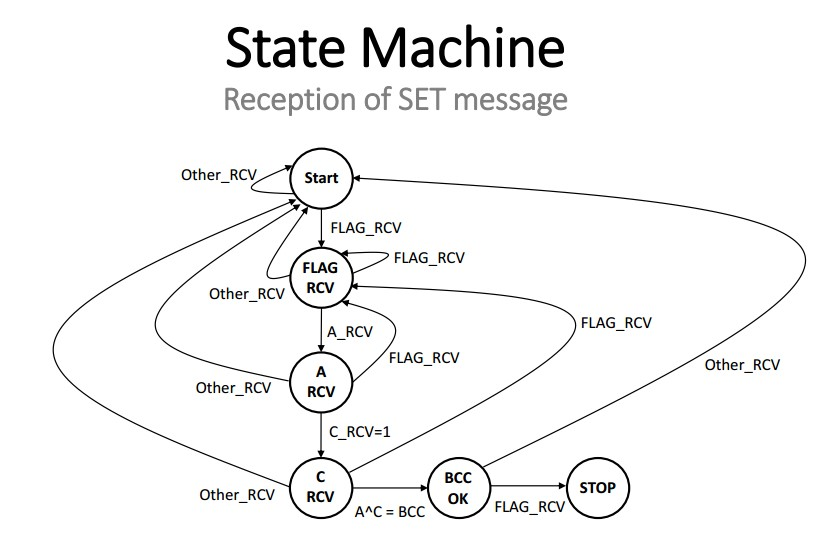
\includegraphics[width=0.5\textwidth]{statemachine.jpg}
	\caption{State Machine}
	\label{Image: State Machine}
\end{figure}

\begin{lstlisting}
while (FALSE == STOP && !timeExceeded) {       /* loop for input */

		printf("Waiting for message...\n");
		
		//Reads one byte
		res = read(fd, &buf, 1);
		
		//State Machine
		if(1 == res) {
			
			if(buf == FLAG) {
				if(s == bcc) s = stop;
				else s = flag; 
			}
			else if(s == flag && (buf == A_TR || buf == A_RT)) {
				s = a;
			}
			else if(s == a && (buf == C_SET || buf == C_UA || (buf & 0x0F) == C_RR || (buf & 0x0F) == C_REJ || buf == C_DISC)) {
				s = c;
			}
			else if(s == c && buf == (message[1]^message[2])) {
				s = bcc;
			}
			else{
				s = start;
				printf("Received something else.\n");
			}

			if (s == flag) n = 0;
			else if(s == a) n = 1;
			else if(s == c) n = 2;
			else if(s == bcc) n = 3;
			else if(s == stop) n = 4;
			else{};

			if(n >= 0) message[n] = buf;

			if (s == stop) STOP = TRUE;
			
		} else {
			printf("Unable to read message.\n");
			return -1;
		}
	printf("Received 0x%02x 0x%02x 0x%02x 0x%02x 0x%02x\n", message[0], message[1], message[2], message[3], message[4]);	
	}
\end{lstlisting}


\section{Application Protocol}

The application layer contains all the higher-lever protocols. Particularly, this layer opens the port, transfers a file (sending it if it is the transmitter or receiving it if it is the receiver) and closes the port. More specifically, the application layer is responsible for the control packages (start and end) and for the data packages. In the function initializeApplicationLayer (function called in main), the port is opened, the Link Layer is initialized, it then calls send or receive function and closes the port. The following structure functions are used:

\begin{lstlisting}
struct applicationLayer {
    int fd;
    int status; //Connection mode, 0 - Receiver, 1 - Transmitter
    unsigned int messageSize;
    char* fileName;
};

struct applicationLayer* application;

int writeControlPackage(int control, char* fileName, char * fileSize);
int initializeApplicationLayer(char* port, unsigned int messageSize, int retries, int timeout, char* fileName, int status);
int send();
int receive();
\end{lstlisting}

In send function, after the connection is established through Link Layer, the Control Package is written and sent as START package. If no errors occur, the data packages (parts of the file that is being transferred) starts being sent. At the end, the Control Package is written and sent as END package and the connection is finished through Link Layer.

In receive function, after the connection is established through Link Layer, the Control Package is received as START package. If no errors occur, the data packages (parts of the file that is being transferred) starts being received and the file is built. At the end, the Control Package is received as END package and the connection is finished through Link Layer.

\section{Validation}

While the implementation was being done, a lot of tests were done to the program, such as, reception capacity, “pinguim.gif” image sending process. We tested with normal conditions, and after we also tested in case of losing and returning connection. In both situations we had the expected response, overcoming duplicated files and
interruptions in sending packages. Receiving “pinguim.gif” image on the receiver computer was done with success.

\section{Valuing Elements}

This program allows the user to choose the maximum size of the data packages that are going to be sent, how many times the program tries to resend packages in case of error, and even the time it waits to retry it. If any error (through BCC) is detected in a frame and it is a frame that has not been sent before, the receiver send a REJ (reject message) so it can be sent again. The program also checks the size of the file received and compares it to the size of the file sent. If any error that disables the file to be transferred entire and correctly occurs, the program is finished and error is reported to the user.

\section{Conclusion}
The data transfer between two computers can be reduced to 4 main functions which allow to open the serial port, send and read data and close the port. Those functions are implemented in the link layer, called \textbf{llopen}, \textbf{llwrite}, \textbf{llread} and \textbf{llclose}, respectively. The application layer is responsible for reading the file in predetermined sized packages and create a correct data package to send and also responsible for reading those packages and write them in a new file in the receiver machine.

The laboratory guide was a very important tool for the development of this project and with it's help we were able to build a program capable of sending any file between two machines connected through a RS-232 serial port. We verified that sending a file from one machine to another is a very complex process and it's necessary to deal with a lot of possible errors that might occur during the transfer. 

In sum, this project contributed to a better understanding of the concepts taught in this subject's classes and for a deeper understanding on how serial ports work.

\section{Contributions}

Summary, Introduction and Conclusion were made by Tiago Almeida.

Architecture, Code Structure and Use Cases were made by Mónica Fernandes and Tiago Almeida.

Link Layer Protocol and Validation were made by João Fidalgo and Carolina Centeio.

Application Protocol and Valuing Elements were made by Carolina Centeio.

\newpage
\clearpage
\vspace*{\fill}
\begin{center}
\begin{minipage}{0.5\textwidth}
\title{\Huge\textbf{Attachment}}
\end{minipage}
\end{center}
\vfill % equivalent to \vspace{\fill}
\clearpage
\newpage

\section{Lab1.c}
\begin{lstlisting}
#include "ApplicationLayer.h"

int main(int argc, char** argv) {

    if(argc != 7) {
        printf("Number of Arguments Wrong: string port, int messageSize, int retries, int timeout, string fileName, int status\n");
        return -1;
    }
	
    char* port = argv[1];
    int messageSize = atoi(argv[2]);
    int retries = atoi(argv[3]);
    int timeout = atoi(argv[4]);
    char* fileName = argv[5];
    int status = atoi(argv[6]);

    //Application Layer function
    initializeApplicationLayer(port, messageSize, retries, timeout, fileName, status);

    return 0;
}
\end{lstlisting}
\newpage

\section{ApplicationLayer.h}
\begin{lstlisting}
#include "LinkLayer.h"

struct applicationLayer {
    int fd;
    int status; //Connection mode, 0 - Receiver, 1 - Transmitter
    unsigned int messageSize;
    char* fileName;
};

struct applicationLayer* application;

int writeControlPackage(int control, char* fileName, char * fileSize);
int initializeApplicationLayer(char* port, unsigned int messageSize, int retries, int timeout, char* fileName, int status);
int send();
int receive();
\end{lstlisting}
\newpage

\section{ApplicationLayer.c}
\begin{lstlisting}
#include "ApplicationLayer.h"

int writeControlPackage(int control, char* fileName, char* fileSize) {

    // C T1 L1 V1(fileSize) T2 L2 V2(fileName) 
    unsigned int controlPackageSize = 5 + strlen(fileSize) + strlen(fileName);

	//Initializes control package variable
    char controlPackage[controlPackageSize];

	//for loop counter
    int i;
    
    //C 2: Start; 3: End
    controlPackage[0] = control;
    
    //T1 - SIZE(0)
    controlPackage[1] = 0; 

    //L1 - Size of V1 field
    controlPackage[2] = strlen(fileSize);

    //Copies the file size to the V1 field
    for (i = 0; i < strlen(fileSize); i++)
        controlPackage[i + 3] = fileSize[i];

    //T2 NAME(1)
    controlPackage[3 + strlen(fileSize)] = 1;
    
    //L2 - Size of V2 field
    controlPackage[4 + strlen(fileSize)] = strlen(fileName);

    //Copies the file name to the V2 field
    for (i = 0; i < strlen(fileName); i++)
        controlPackage[5 + strlen(fileSize) + i] = fileName[i];

    //llwrite - LinkLayer function 
    return llwrite(application->fd, controlPackage, controlPackageSize);
}

int initializeApplicationLayer(char* port, unsigned int messageSize, int retries, int timeout, char* fileName, int status) {

	//Allocates memory for application struct
	application = (struct applicationLayer*) malloc(sizeof(struct applicationLayer));

	//Opens the port and stores the file descriptor in the application structure
	application->fd = open(port, O_RDWR | O_NOCTTY );

	//Stores the messageSize in the application structure
	application->messageSize = messageSize;

	//Checks if the port was successfully opened
	if (application->fd < 0) {
		printf("Unable to opening port.\n");
		return -1;
	}

	//Stores the mode of the computer: 0 - Receiver, 1 - Transmitter
	application->status = status;

	//Stores the file name in the application structure
	application->fileName = fileName;

	//Initializes link layer
	if(initializeLinkLayer(application->fd, port, retries, timeout) < 0) {
		printf("Unable to initialize link layer.\n");
		return -1;
	}

	//Checks if the computter is in transmitter mode
	if(application->status == TRANSMITTER)
		send();
	//Checks if the computer is in receiver mode
	else if(application->status == RECEIVER)
		receive();
	//Else nothing happens, simply closes the port

	//Restores the termios
	if (tcsetattr(application->fd, TCSANOW, &oldtio) == -1) {
		perror("tcsetattr");
		return -1;
	}

	//Closes the port
	close(application->fd);

	free(application);
	return 0;
}

int send(){

	printf("Start writing\n");
	//Opens the file as a binary file for reading
	FILE* file = fopen(application->fileName, "rb");
	if(!file) {
		//Debug: Error message when unable to open file.
		printf("Unable to open the specified file.\n");
		return -1;
	}

	//Places the file pointer at the end of the file
	fseek(file, 0, SEEK_END);
	
	//For binary streams, this is the number of bytes from the beginning of the file.
	unsigned int fileSize = ftell(file);

	//Places the file pointer at the beginning of the file
	fseek(file, 0, SEEK_SET);
	
	//Declaration of the array that will store the file size
	char sizeString[10];

	//Transforms the size of the file into a string
	sprintf(sizeString, "%u", fileSize);
	
	//Degub: Prints the file size
	printf("File size: %u Bytes.\n", fileSize);

	//Tries to establish connection by sending the C_SET command
	if(llopen(application->fd, application->status) < 0)
		return -1;
		
	//Sends the start package to the receiver, 2: START
	if(writeControlPackage(2, application->fileName, sizeString) < 0) {
		//Debug: Error message when unable to send start control package
		printf("Unable to send start control package.\n");
		return -1;
	}
	
	//Debug: Message when sending process starts
	printf("Starting sending...\n");
	
	//Variable to store the number of bytes read per iteration
	unsigned int bytesRead;
	
	//C N L2 L1 P(messageSize)
	unsigned char* data = (unsigned char*)malloc((application->messageSize + 4) * sizeof(unsigned char));

	//Initializes the data package sequence number
	unsigned int packageSequenceNumber = 0;
	
	//Iteration that reads while there is something to read
	while((bytesRead = fread(data + 4, sizeof(char), application->messageSize, file)) > 0) {

		//C - Data which is represented as the number 1
		data[0] = 1;

		//N - Package sequence number
		data[1] = (packageSequenceNumber % 255);

		printf("Data package %d.\n", data[1]);
		
		//L2 - bytes / 256
		data[2] = bytesRead >> 8;
		
		//L1 - bytes % 256
		data[3] = bytesRead & 0xFF;
		
		//Calls the LinkLayer function to send the data
		if(llwrite(application->fd, (char*)data, bytesRead + 4) == -1) {
			//Debug: Error message when unable to send data package
			printf("Unable to write package %d.\n", packageSequenceNumber);
			return -1;
		}
		
		//Updates the package sequence number
		packageSequenceNumber++;
	}

	free(data);
	
	//Closes the file
	if (fclose(file) != 0) {
	
		//Debug: Error message when unable to close file
		printf("Unable to close file.\n");
		return -1;
	}
	
	//Sends the end package to the receiver, 3 - END
	if(writeControlPackage(3, application->fileName, sizeString) < 0) {
		
		//Debug: Error message when unable to send end package
		printf("Unable to send end package.\n");
		return -1;
	}
		
	//Calls close function from Linklayer
	if(llclose(application->fd, application->status) < 0)
		return -1;
	
	printf("\n");
	return 0;
}

int receive(){

	//Tries to establish connection by reading the C_UA response
	if(llopen(application->fd, application->status) <= 0)
		return -1;

	//Variable initialization
	FILE* file = NULL; 
	char fileName[30] = "";
	char fileSize[10] = "";
	unsigned char package[3000];

   	memset(package, 0, 3000);

	int received = 0;

	while(0 == received){
		
		int dataSize = llread(application->fd, (char*)package);
		
		//If llread didn't fail reading the data package	
		if(dataSize > 0) {

			//If the package received is the end package
			if(3 == package[0])
				received = 1;
			
			//if the package received is the start package
			if(2 == package[0]) {

				//i starts at 1, because the first position was already tested
				int i = 1;
				while(i < dataSize) {

					int j = 0;
					
					//If the next section of the data package is representing the file size
					if(0 == package[i]) {

						printf("Reading file size.\n");
						for(; j < package[i+1]; j++) { // i+1 = V length
							fileSize[j] = package[j+i+2];
						}
					}
					//If the next section of the data package is representing the file name
					else if(1 == package[i]) {

						printf("Reading file name.\n");
						for(; j < package[i+1]; j++) { 
							fileName[j] = package[i+j+2];
						}
					}
					//i moves to the next T position, T2 i(C) += j(V) + 2(T1 + L1)
					i += j + 2;					
				}

				//Creates a new file with the name sent by the transmitter
				if((file = fopen(fileName, "wb")) < 0){
					printf("Unable to open the file.\n");
					return -1;
				}
			}

			//If the package received is a data package
			if(1 == package[0] && file != NULL) { 
				printf("Writing to the file.\n");
				//Prints the data package sequence number
				printf("Data package: %d.\n", package[1]);
				int psize = (unsigned char)package[2] << 8 | (unsigned char)package[3]; //(K = 256*L2+L1)
				fwrite(&package[4], sizeof(char), psize, file);
			}
		}

		//Reset the package information to zero to prevent "garbage" data
		memset(package, 0, 3000);
	}

	//Closes the file that was transfered
	if (fclose(file) < 0){
		printf("File %s was not closed.\n", fileName);
		return -1;
	}	

	//Closes the port
	if (llclose(application->fd, application->status) < 0) {
		printf("Serial port was not closed. \n");
		return -1;
	}

	printf("File transfered successfully.\n");
	
	printf("Size of the received file: %s.\n", fileSize);
	return 0;
}
\end{lstlisting}
\newpage

\section{LinkLayer.h}
\begin{lstlisting}
#include <sys/types.h>
#include <sys/stat.h>
#include <fcntl.h>
#include <termios.h>
#include <stdio.h>
#include <signal.h>
#include <stdlib.h>
#include <string.h>
#include <fcntl.h>
#include <unistd.h>

#define BAUDRATE B38400
#define MODEMDEVICE "/dev/ttyS1"
#define _POSIX_SOURCE 1 /* POSIX compliant source */
#define FALSE 0
#define TRUE 1
#define FLAG 0x7e
#define ESCAPE 0x7d
#define A_TR 0x03
#define A_RT 0x01
#define C_SET 0x03
#define C_UA 0x07
#define C_REJ 0x01
#define C_RR 0x05
#define C_DISC 0x0B
#define RECEIVER 0
#define TRANSMITTER 1
#define SUPERVISIONPACKAGE 5

struct linkLayer {
    char port[20];
    unsigned int sequenceNumber;
    unsigned int timeout;
    unsigned int triesMAX;
};

enum STATE{
	start,
	flag,
	a,
	c,
	bcc,
	stop
} state;

struct linkLayer* llink;
struct termios oldtio,newtio;

unsigned int timeExceeded;

void handleAlarm();
int sendMessage(int fd, char* message);
int receiveMessage(int fd, char* message);
int initializeLinkLayer(int fd, char * port, int triesMAX, int timeout);
int llopen(int fd, int connectionMode);
int llwrite(int fd, char* buffer, unsigned int length);
int llread(int fd, char* buffer);
int llclose(int fd, int mode);
unsigned int dataStuffing(char* buffer, unsigned int frameSize);
unsigned int dataDestuffing(char* buffer, unsigned int frameSize);
char findBCC2(char* data, unsigned int size);
\end{lstlisting}
\newpage

\section{LinkLayer.c}
\begin{lstlisting}
#include "LinkLayer.h"

void handleAlarm() {
	timeExceeded = 1;
	printf("Alarm called.\n");
 }

int sendMessage(int fd, char* message) {
	//Debug: Prints message to send
	printf("Sending 0x%02x 0x%02x 0x%02x 0x%02x 0x%02x\n", message[0], message[1], message[2], message[3], message[4]);
	
	//Sends the message to the port and return the number of bytes read
	return write(fd, message, SUPERVISIONPACKAGE * sizeof(char));
}

int receiveMessage(int fd, char* message) {
	char buf;
	int res;
	int STOP = FALSE;
	int n = -1;
	enum STATE s = start;

	while (FALSE == STOP && !timeExceeded) {       /* loop for input */

		printf("Waiting for message...\n");
		
		//Reads one byte
		res = read(fd, &buf, 1);
		
		//State Machine
		if(1 == res) {
			
			if(buf == FLAG) {
				if(s == bcc) s = stop;
				else s = flag; 
			}
			else if(s == flag && (buf == A_TR || buf == A_RT)) {
				s = a;
			}
			else if(s == a && (buf == C_SET || buf == C_UA || (buf & 0x0F) == C_RR || (buf & 0x0F) == C_REJ || buf == C_DISC)) {
				s = c;
			}
			else if(s == c && buf == (message[1]^message[2])) {
				s = bcc;
			}
			else{
				s = start;
				printf("Received something else.\n");
			}

			if (s == flag) n = 0;
			else if(s == a) n = 1;
			else if(s == c) n = 2;
			else if(s == bcc) n = 3;
			else if(s == stop) n = 4;
			else{};

			if(n >= 0) message[n] = buf;

			if (s == stop) STOP = TRUE;
			
		} else {
			printf("Unable to read message.\n");
			return -1;
		}
	printf("Received 0x%02x 0x%02x 0x%02x 0x%02x 0x%02x\n", message[0], message[1], message[2], message[3], message[4]);	
	}
	
	return 0;
}

int initializeLinkLayer(int fd, char * port, int triesMAX, int timeout) {
	
	//Allocates memory for the linkLayer structure
	llink = (struct linkLayer*)malloc(sizeof(struct linkLayer));
	
	//Initializes link layer structure
	strcpy(llink->port, port);
	llink->timeout = timeout;
	llink->triesMAX = triesMAX;
	llink->sequenceNumber = 0;
    
    //Set up alarm routine
	(void) signal(SIGALRM, handleAlarm);
	
	//Changes the termios settings
	if (tcgetattr(fd, &oldtio) == -1) { /* save current port settings */
      perror("tcgetattr");
      return -1;
    }

    bzero(&newtio, sizeof(newtio));
    newtio.c_cflag = BAUDRATE | CS8 | CLOCAL | CREAD;
    newtio.c_iflag = IGNPAR;
    newtio.c_oflag = 0;

    /* Set input mode (non-canonical, no echo,...) */
    newtio.c_lflag = 0;

    newtio.c_cc[VTIME]    = 10;   /* inter-character timer unused */
    newtio.c_cc[VMIN]     = 0;   /* blocking read until 5 chars received */



    tcflush(fd, TCIOFLUSH);

    if (tcsetattr(fd, TCSANOW, &newtio) == -1) {
      perror("tcsetattr");
      return -1;
    }

    printf("New termios structure set\n");
	return 0;
}


int llopen(int fd, int status) {
	int counter = 0, isConnected = FALSE;

	if(TRANSMITTER == status) {
		while(isConnected == FALSE) {
			
			//Only retries to send the frame if the time was Exceeded
			if(counter == 0 || timeExceeded) {
				timeExceeded = 0;
				
				//If the number of tries was exceeded
				if(counter >= llink->triesMAX) {
					printf("Unable to establising connection.\n");			
					return -1;
				}
			
				//Builds the set frame
				char* setPackage = (char*)malloc(SUPERVISIONPACKAGE * sizeof(char));
				setPackage[0] = FLAG;
				setPackage[1] = A_TR;
				setPackage[2] = C_SET;
				setPackage[3] = setPackage[1] ^ setPackage[2];
				setPackage[5] = FLAG;
			
				//Sends the set frame
				sendMessage(fd, setPackage);
				free(setPackage);
		
				counter++;
				alarm(llink->timeout);
			}
			
			//Allocates memory to receive the message
			char* receivedMessage = (char*)malloc(SUPERVISIONPACKAGE * sizeof(char));
		
			//If a message was read
			if(receiveMessage(fd, receivedMessage) != -1) {
				//If the message is UA, the connection between the two computers is online
				if(receivedMessage[1] == A_TR && receivedMessage[2] == C_UA) {
					alarm(0);
					printf("Connection established.\n");
					isConnected = TRUE;
				}		
			}
			free(receivedMessage);
		}
		timeExceeded = 0;
	} else {
		while(isConnected == FALSE) {
			
			//Allocates memory to receive the set frame
			char* setPackage = (char*)malloc(SUPERVISIONPACKAGE * sizeof(char));
			
			//Reads the message from the port
			receiveMessage(fd, setPackage);

			//If the message is SET
			if(setPackage[1] == A_TR && setPackage[2] == C_SET) {

				//Builds the frame UA to send
				char* uaPackage = (char*)malloc(SUPERVISIONPACKAGE * sizeof(char));

				uaPackage[0] = FLAG;
				uaPackage[1] = A_TR;
				uaPackage[2] = C_UA;
				uaPackage[3] = uaPackage[1] ^ uaPackage[2];
				uaPackage[4] = FLAG;

				//Sends the UA frame
				sendMessage(fd, uaPackage);
				free(uaPackage);
				
				isConnected = TRUE;
				printf("Connection established.\n");
      		}
			free(setPackage);
		}
	}
	return fd; 
}

int llwrite(int fd, char* buffer, unsigned int length) {

	//6 for the F, A, C, BCC1, BCC2 and F
	char* frame = (char*)malloc(length + 6 * sizeof(char));
	
	//Creates the BBC2 flag depeding on the data
	char BCC2 = findBCC2(buffer, length);
	
	//Builds the frame to send
	frame[0] = FLAG;
	frame[1] = A_TR;
	frame[2] = (llink->sequenceNumber << 6);
	frame[3] = frame[1]^frame[2];
	memcpy(&frame[4], buffer, length);
	frame[4 + length] = BCC2;
	frame[5 + length] = FLAG;

	//Data stuffing
	int newSize = dataStuffing(frame, length + 6 * sizeof(char));

	int STOP = FALSE;
	int counter = 0;

	while(!STOP){
		
		//It only retries to send the code if the time was exceeded
		if(counter == 0 || timeExceeded){
			timeExceeded = 0;
			//If the number of tries was exceeded
			if (counter >= llink->triesMAX) {
				printf("Unable to send data package.\n");
				return -1;
			}
			
			printf("%x, %x, %x, %x.\n", frame[0], frame[1], frame[2], frame[3]);
			//Sends Information frame
			if(write(fd, frame, newSize) == -1){
				printf("Unable to write data package\n");
				return -1;
			}
			counter++;
			alarm(llink->timeout);
		}

		char response[SUPERVISIONPACKAGE];

		receiveMessage(fd, response);
		
		if(response[0] == FLAG && response[1] == A_TR) {
			
			//If the Information frame was rejected
			if((response[2] & 0x0F) == C_REJ) {
				printf("REJ\n");

				//If the sequence number is the same as the one sent, retry to send the Information frame
				if((response[2] >> 7) == llink->sequenceNumber) {
				  alarm(0);
				  counter = 0;
				}

				//If the sequence number is not the same, the response was not correctly built
				else {
				  printf("REJ response was not correctly built.\n");
				  return -1;
				}
			}

			else if ((response[2] & 0x0F) == C_RR) {
				printf("RR\n");
				
				//If the sequence number is not the same as the one sent, the frame was accepted 
				if((response[2] >> 7) != llink->sequenceNumber) {
					alarm(0);
					llink->sequenceNumber = (response[2] >> 7);
					STOP = TRUE;
				}

				//The header of the package was accepted, but the data field needs to be resent
				else {
					
					//Sets timeExceeded to 1 to be able to resend the Information frame
					handleAlarm();
				}
			}
		}
	}
	
	free(frame);
	//Reset timeExceeded flag
	timeExceeded = 0;

	return newSize;
}

int llread(int fd, char* buffer) {
	int STOP = FALSE;

	//0 - Before receiving the first FLAG flag | 1 - After receiving the first FLAG flag and before receiving the last FLAG flag || 2 - After receiving the last
	// FLAG flag
	int state = 0;
	int size = 0;

	char* buff = (char*)malloc(3000);

	while(!STOP){

		char c;
		if(state < 2) {
			int res = read(fd, &c, 1);
			if(res == -1){
				printf("Unable to read Information package.\n");
				return -1;
			}
		}

		switch(state){
			case 0:
				if(c == FLAG) {
					buff[size] = c;
					size++;
					state = 1;
				}
				break;
			case 1:
				if(c == FLAG && size != 1) {
					buff[size] = c;
					size++;
					state = 2;
				}

				else if(c == FLAG && size == 1){;}

				else {
					buff[size] = c;
					size++;
				}
				break;
			default:
				STOP = TRUE;
				break;
		}
	}

	printf("Received 0x%x 0x%x 0x%x 0x%x.\n", buff[0], buff[1], buff[2], buff[3]);
	int process = FALSE;
	int newSize = dataDestuffing(buff, size);

	if(buff[0] != FLAG || buff[1] != A_TR || buff[3] != (buff[1] ^ buff[2])){
		printf("Received frame header was not corretly built\n");
		free(buff); 
		return -1;
	}

	//6 - F, A, C, BCC1, BCC2 and F
	int dataPackageSize = newSize - 6 * sizeof(char);

	//Creates BCC2 depending on the data field
	char BCC2 = findBCC2(&buff[4], dataPackageSize);
	
	//Only the last bit is considered
	unsigned int sequenceNumber = (buff[2] >> 6) & 1;

	char response[SUPERVISIONPACKAGE * sizeof(char)];
	response[0] = FLAG;
	response[1] = A_TR;
	response[4] = FLAG;

	//If the right frame was received (With the expected sequence number)
	if(llink->sequenceNumber == sequenceNumber) {

		//If the data BBC does not match, the frame was corrupted
		if(BCC2 != buff[newSize - 2]) {
			printf("Data BCC does not match the data BCC received.\nFrame rejected.\n");
			response[2] = (llink->sequenceNumber << 7) | C_REJ;
		}
		else {
			//Updates the sequenceNumber to the next one
			if(llink->sequenceNumber == 0) {
				llink->sequenceNumber = 1;
			}
		  	else {
		  		llink->sequenceNumber = 0;
		  	}
		  	process = TRUE;
			
			//Sends RR as a response			  	
			response[2] = (llink->sequenceNumber << 7) | C_RR;
	  }
	}
	else{
		//If it's duplicate, send RR response with the same sequence number that was updated when the frame was received the first time
		response[2] = (llink->sequenceNumber << 7) | C_RR;
	}

	//BCC1
	response[3] = response[1]^response[2];
	
	//Sends the response
	sendMessage(fd, response);
	
	//If the Information frame was accepted 
	if(process) {

		//Updates the argument buffer to contain the data
		memcpy(buffer, &buff[4], dataPackageSize);
		free(buff);
		return dataPackageSize;
	}

	free(buff);
	return -1;
}

int llclose(int fd, int mode){
	printf("Closing\n");
	int disc = 0, counter = 0;

	if(TRANSMITTER == mode){
		while(0 == disc) {

			//Only retries to send the frame if the time was exceeded
			if(counter == 0 || timeExceeded) {
				timeExceeded = 0;
				//If the number of tries was exceeded
				if(counter >= llink->triesMAX) {
					printf("Unable to disconnect.\n");			
					return -1;
				}
			
				//Allocates memory for the disconnect frame
				char* discPackage = (char*)malloc(SUPERVISIONPACKAGE * sizeof(char));				
				
				//Builds the disconnect frame
				discPackage[0] = FLAG;
				discPackage[1] = A_TR;
				discPackage[2] = C_DISC;
				discPackage[3] = (discPackage[1]^discPackage[2]);
				discPackage[4] = FLAG;

				//Sends the disconnect frame
				if(sendMessage(fd, discPackage) < 0) {
					printf("Unable to send disconnect frame.\n");
					return -1;
				}

				free(discPackage);
				alarm(llink->timeout);
				
				//Updates the number of tries
				counter++;
			}
			
			//Allocates space for the response
			char* response = (char*)malloc(SUPERVISIONPACKAGE * sizeof(char));
		
			//Reads the response
			if(receiveMessage(fd, response) < 0) {
				printf("Unable to read disconnect response.\n");
				return -1;				
			}

			//If the received frame is the disconnect frame, it disconnected successfully
			if(response[1] == A_RT && response[2] == C_DISC) {
				disc = 1;
				
				//Allocates space for the response (UA)
				char* UA = (char*)malloc(SUPERVISIONPACKAGE * sizeof(char));				

				//Builds the UA frame to respond
				UA[0] = FLAG;
				UA[1] = A_RT;
				UA[2] = C_UA;
				UA[3] = (UA[1]^UA[2]);
				UA[4] = FLAG;

				//Sends the UA frame as a response
				if(sendMessage(fd, UA) < 0) {
					printf("Unable to write UA frame as a response to disconnect.\n");
					return -1;					
				}
				
				free(UA);
				printf("Disconnected.\n");
			}
			free(response);
		}
		alarm(0);
		sleep(3);
	}
	else if(RECEIVER == mode) {
		
		//Allocates memory for the disconnect frame read from the transmitter
		char* discPackage = (char*)malloc(SUPERVISIONPACKAGE * sizeof(char));				
		
		//Reads the disconnect frame
		if(receiveMessage(fd, discPackage) < 0){
			printf("Unable to receive disconnect package from transmitter.\n");
			return -1;				
		}				
	
		//If the frame received is the disconnect frame
		if(discPackage[1] == A_TR && discPackage[2] == C_DISC) {

			//While it's not disconnected
			while(0 == disc) {

				//It only resends if the time has exceeded
				if (counter == 0 || timeExceeded) {
					timeExceeded = 0;

					if (counter >= llink->triesMAX) {
						printf("Unable to disconnect.\n");
						return -1;
					}

					//Allocates memory for the disconnect response
					char* response = (char*)malloc(SUPERVISIONPACKAGE * sizeof(char));				

					//Builds the disconnect response
					response[0] = FLAG;
					response[1] = A_RT;
					response[2] = C_DISC;
					response[3] = (response[1]^response[2]);
					response[4] = FLAG;

					//Sends the disconnect frame as a response
					if(sendMessage(fd, response) < 0) {
						printf("Unable to send disconnect frame as a response.\n");
						return -1;					
					}

					free(response);
					counter++;
					alarm(llink->timeout);
				}

				//Allocates memory for the UA response from the transmitter
				char* UA = (char*)malloc(SUPERVISIONPACKAGE * sizeof(char));

				//Reads the UA response
				if(receiveMessage(fd, UA) < 0) {
					printf("Unable to read the UA response from the transmitter\n");
					return -1;				
				}

				//If the UA response is accepted
				if(UA[1] == A_RT && UA[2] == C_UA) {
					disc = 1;
					free(UA);
					printf("Disconnected.\n");
				}
			}
		}
		free(discPackage);			
	}

	free(llink);
	return 0;
}

unsigned int dataStuffing(char* buffer, unsigned int frameSize) {
	unsigned int newframeSize = frameSize;

	//i = 1 Starts at 1 because the initial flag must remain intact 
	//i < frameSize - 1 because the last flag must remain intact
	int i;
	for (i = 1; i < frameSize - 1; i++)
	
		//FLAG = 0x7e ESCAPE = 0x7d
		if (buffer[i] == FLAG || buffer[i] == ESCAPE)
			newframeSize++;
	
	//Reallocates memory for the buffer, adding more space in the end		
	buffer = (char*) realloc(buffer, newframeSize);
	
	for (i = 1; i < frameSize - 1; i++) {
	
		if (buffer[i] == FLAG || buffer[i] == ESCAPE) {
		
			//Moves everything from position i in the buffer one position ahead
			memmove(buffer + i + 1, buffer + i, frameSize - i);
			frameSize++;
			
			//Set the i position, where last was the FLAG or ESCAPE and replaces it with the ESCAPE flag
			buffer[i] = ESCAPE;
			
			//Applies exclusive or to the flag that needs to be substituted
			buffer[i + 1] ^= 0x20;
		}
	}
	
	//Returns the frase after stuffing mechanism
	return newframeSize;
}

unsigned int dataDestuffing(char* buffer, unsigned int frameSize){

	int i;
	for (i = 1; i < frameSize - 1; i++) {
		//ESCAPE = 0x7d
		if (buffer[i] == ESCAPE) {
		
			//Moves the array one position to the left, eliminating the ESCAPE flag
			memmove(buffer + i, buffer + i + 1, frameSize - i - 1);
			frameSize--;
			
			//Applies exclusive or to the flag to restore the previous byte
			buffer[i] ^= 0x20;
			
		}
	}
	
	//Reallocates memory deleting the last position that are not part of the original frame
	buffer = (char*) realloc(buffer, frameSize);

	//Returns the size of the original frame
	return frameSize;
	
}

char findBCC2(char* data, unsigned int size) {
	int i;
	char BCC2 = 0;
	
	//Iterates through the data buffer and apply the exclusive or to all the elements
	for(i = 0; i < size; i++) {
		BCC2 ^= data[i];
	}

	return BCC2;
}
\end{lstlisting}

\end{document}
